%
%	Configure LaTeX to produce a PDF presentation using the beamer class
%


% Default is 16:9 widescreen ratio
\documentclass[ignorenonframetext,12pt,aspectratio=169]{beamer}

% For 4:3 ratio use this:
% \documentclass[ignorenonframetext,11pt]{beamer}


%\documentclass[onesided]{article}
%\usepackage{graphicx}
%\usepackage{beamerarticle}

\usepackage{beamerthemesplit}
\usepackage{patchcmd}
\usepackage{tabulary}		% Support longer table cells
\usepackage{booktabs}		% Support better tables
\usepackage[sort&compress]{natbib}
\usepackage{acronym}			% Support acronyms
\usepackage{listings}			% Allow for source code highlighting

\usepackage{framed}			% Allow background color for images
\definecolor{shadecolor}{named}{white}


\usepackage{subfigure}

\let\oldSubtitle\subtitle


% Configure default metadata
%
%	Configure default metadata in case it's missing to avoid errors
%

\def\myauthor{Author}
\def\defaultemail{}
\def\defaultposition{}
\def\defaultdepartment{}
\def\defaultaddress{}
\def\defaultphone{}
\def\defaultfax{}
\def\defaultweb{}
\def\defaultaffiliation{}

\def\mytitle{Title}
\def\subtitle{}
\def\mykeywords{}


\def\bibliostyle{plain}
% \def\bibliocommand{}

\def\myrecipient{}

% Overwrite with your own if desired
%\input{ftp-metadata}




\AtBeginSection[]
{
   \begin{frame}
       \frametitle{Outline}
       \tableofcontents[currentsection,currentsubsection]
   \end{frame}
}


\long\def\citefoot#1{\let\thefootnote\relax\footnotetext{\citet{#1}} }


%
%	Get ready for the actual document
%

%
% Use default MMD metadata for beamer equivalents
%

\ifx\subtitle\undefined
\else
	\oldSubtitle{\subtitle}
\fi

\ifx\affiliation\undefined
\else
	\institute{\affiliation}
\fi

\ifx\mydate\undefined
	\def\mydate{\today}
\else
	\date{\mydate}
\fi

\ifx\event\undefined
\else
	\date[\mydate]{\mydate~ / \event }
\fi


%\input{mmd-title}

% Show "current/total" slide counter in footer
\title[\mytitle\hspace{2em}\insertframenumber/
\inserttotalframenumber]{\mytitle}


\author{\myauthor}
\addtolength{\parskip}{\baselineskip}

\ifx\theme\undefined
\else
	\usetheme{\theme}
\fi

\begin{document}
\frame{\setlength\parskip{0pt}\titlepage}


    \begin{abstract}
        As most research papers have an abstract, there are predefined commands for telling LaTeX which part of the content makes up the abstract.
        This should appear in its logical order, therefore, after the top matter, but before the main sections of the body.
        This command is available for the document classes article and report, but not book.
    \end{abstract}

    \section{Introduction}
    Hello World!

    \section{Figures and Tables}
        Taken from \url{https://en.wikibooks.org/wiki/LaTeX/Floats,_Figures_and_Captions}.

        \begin{figure}
          \caption{A picture of a gull.}
          \centering
            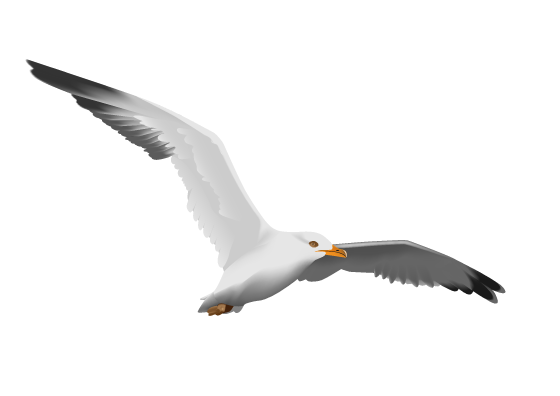
\includegraphics[width=0.5\textwidth]{gull}
        \end{figure}

        \begin{figure}
          \centering
            \reflectbox{%
              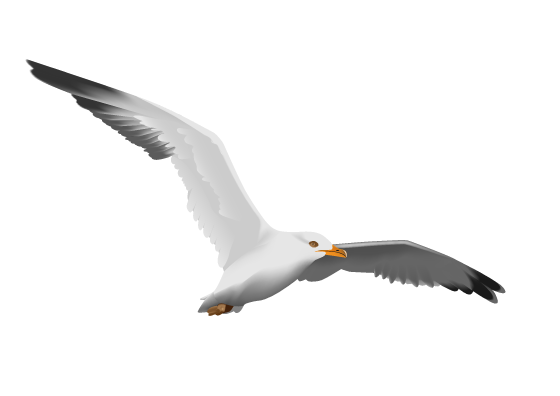
\includegraphics[width=0.5\textwidth]{gull}}
          \caption{A picture of the same gull looking the other way!}
        \end{figure}

        \begin{table}
          \centering
            \begin{tabular}{| l c r |}
            \hline
            1 & 2 & 3 \\
            4 & 5 & 6 \\
            7 & 8 & 9 \\
            \hline
            \end{tabular}
          \caption{A simple table}
        \end{table}

        Notice how the tables and figures have independent counters.

    \subsection{Math}

        \begin{equation}
            e = mc^2
        \end{equation}

        \begin{equation}
            \nabla \cdot \sigma + \mathbf{b} = \mathbf{0}
        \end{equation}

%
%	MultiMarkdown beamer class footer file
%

% Back Matter
\if@mainmatter
\backmatter
\fi

\ifx\bibliocommand\undefined
\else
	\part{Bibliography}
	\begin{frame}[allowframebreaks]
	\frametitle{Bibliography}
	\bibliographystyle{\bibliostyle}
	\def\newblock{}
	\bibliocommand
	\end{frame}
\fi


\end{document}
